\documentclass[11pt]{article}
\textheight 22cm \textwidth 16.5cm \oddsidemargin 0cm \topmargin -.5cm
\usepackage[utf8x]{inputenc}
\usepackage{pricing_notes}

\date{Lecture 4 (29 Jan. 2013)}

\begin{document}

{\small \maketitle}

\section{Recapitulation}

Let $\widetilde{\Phi}_T$ denote an attainable\footnote{With at least one replicating portfolio built from primitive securities.} contingent claim paying a unique cashflow at date $T$. Recall that its value under stocastic interest rates is:
$$ V_t(\widetilde{\Phi}_T) = \Exp_{\Qmeas} \left[ \widetilde{\Phi}_T e^{-\int_t^T r(s) ds} \middle/ \Filtr_t \right]$$\\
Recall also that in the case where $\widetilde{\Phi}_T$ is constant (e.g. $\widetilde{\Phi}_T = 1$) then we have:
$$ V_t(\widetilde{\Phi}_T) = \Exp_{\Qmeas} \left[ 1 \cdot e^{-\int_t^T r(s) ds} \middle/ \Filtr_t \right] = B^T(t)$$\\
where $B^T$ are short-term bonds, and by definition
$$B^T(t) = \Exp_{\Qmeas} \left[ e^{-\int_t^T r(s) ds} \middle/ \Filtr_t \right]$$
So far we have only worked with $r(t)$, the short term interest rate paid over the short interval $t$ and $t+\Delta t$. We now introduce the spot rate $R(t, \theta)$, the interest rate observed at time $t$ for lending over the period $(t, t+\theta)$, defined as follows:
$$B^T(t) \equiv e^{-(T-t)R(t,T-t)}$$
By observing a collection of zero-coupon bonds on the market, we are able to infer the function of spot rates $R(t, \theta)$ over $\theta$, which we call the {\em yield curve}.
We also observe that the instantaneous short term rate can be defined as the limit of the spot rate as its maturity $\theta$ approaches zero:
$$r(t) = \lim_{\theta \rightarrow 0} R(t, \theta)$$
Finally, we note that the category of instruments where $\widetilde{\Phi}_T$ is constant are what we call fixed-coupon bonds. We consider them to be default-free (i.e., no credit risk), and of certain payoff. Since there are no random cash flows, they are easy to price, and the market price is the no-arbitrage price. \\

The world of interest-rate-linked securities is often referred to as the {\em fixed income} market. It includes other instruments such as floating rate notes (notes with variable payments), caplets (options on interest rates), caps (collections of caplets), options on bonds. When pricing such instruments, whose cash flows depend on the evolution of interest rates, we cannot assume constant interest rates. \\

\begin{remark}
By its nature, the problem of interest rates is much more complicated than equities. When pricing an option on a stock, the only thing I am interested in is the single price process $\left\{S(t)\right\}_{t \geq 0}$. For Bachelier, this was arithmetic Brownian motion; for Black and Scholes, it was geometric Brownian motion; it can also be a pure-jump Lévy process, as in (Geman 2002).\\ 

In the problem of interest rates, we consider the yield curve and its evolution into the future, $\left\{ R(t, \theta), \theta > 0 \right\}_{t \geq 0}$, which is an infinite dimensional system. From empirical observation, we can also observe that there are no pricing anomalies in the zero-coupon bond market, and therefore our model and the dynamics of the yield curve must also be consistent with the principle of no arbitrage.
\end{remark}

\section{Review: Change of Measure for Stochastic Interest Rates}


Recall that last week we introduced a new probability measure to take the interest rate term $e^{-\int_t^T r(s) ds}$ out of the expectation, by constructing the Radon-Nikodym derivative
$$\frac{\dif \Qmeas_T}{\dif \Qmeas} = \frac{e^{-\int_t^T r(s) ds}}{B^T(t)}$$
which we defined in such as way as to have an expected value of 1 under the original probability measure $\Qmeas$. From our original expression, 
\begin{align*}
V_t(\widetilde{\Phi}_T)
&= \Exp_{\Qmeas} \left[ \widetilde{\Phi}_T e^{-\int_t^T r(s) ds} \middle/ \Filtr_t \right]
\intertext{we substitute the derivative:} 
&= \Exp_{\Qmeas} \left[ \widetilde{\Phi}_T B^T(t) \frac{\dif \Qmeas_T}{\dif \Qmeas} \middle/ \Filtr_t \right]
\intertext{The bond price is observed, so we can take it out from under the expectation:}
&= B^T(t) \Exp_{\Qmeas} \left[ \widetilde{\Phi}_T \frac{\dif \Qmeas_T}{\dif \Qmeas} \middle/ \Filtr_t \right]
\intertext{We then invoke measure theory to convert the expectation to the integral,}
&= B^T(t) \int_\Omega \widetilde{\Phi}_T \frac{\dif \Qmeas_T}{\dif \Qmeas} \dif \Qmeas 
\intertext{cancel the $\dif \Qmeas$ term, which is a well defined operation,}
&= B^T(t) \int_\Omega \widetilde{\Phi}_T \dif \Qmeas_T
\intertext{and finally convert the integral over $\dif \Qmeas_T$ back to an expectation to obtain the result:}
V_t(\widetilde{\Phi}_T) &= B^T(t) \Exp_{\Qmeas_T} \left[ \widetilde{\Phi}_T \middle/ \Filtr_t \right]
\end{align*}
Note that we made absolutely no assumptions on what we call the interest rate model. \\

Now let us return to the basic economy with primitive securities (stocks and bonds) denoted $\widetilde{S}_j(t)$ where $s=0,\dots,n$. Let $\widetilde{\Phi}_T$ be the random value today of the stock $\widetilde{S}_j$ time $T$. If the market is indeed arbitrage free, then the value today of the future cash flow $V_t(\widetilde{\Phi}_T)$ is equal the price of the stock today $\widetilde{S}_j(t)$.
$$V_t(\widetilde{\Phi}_T) = \widetilde{S}_j(t) = B^T(t) \Exp_{\Qmeas_T} \left[ \widetilde{S}_j(T) \middle/ \Filtr_t \right] = B^T(t) \Exp_{\Qmeas_T} \left[ \frac{\widetilde{S}_j(T)}{B^T(T)} \middle/ \Filtr_t \right]$$
since $B^T(T) = 1$. This implies that:
$$\frac {\widetilde{S}_j(t)}{B^T(t)} = \Exp_{\Qmeas_T} \left[ \frac{\widetilde{S}_j(T)}{B^T(T)} \middle/ \Filtr_t \right]$$
that is, the $T$-forward price of the stock $\widetilde{S}_j$ is a $\Qmeas_T$-martingale under stochastic interest rates.\\

Now look at the asset that we denote $S_0 = B^T$.
\begin{remark}
Note that under the assumption of constant short-term interest rates we consider the instrument $M$, the money market account growing at rate $r$. In the case of stochstic interest rates we consider instead the instrument $B^T$, the zero-coupon bond, whose price at time $t$ can be observed and the only instrument in the economy whose payoff at time time $T$ is known.
\end{remark}
Consider the value of the zero-coupon bond at time $t$ divided by itself: this is the $T$-forward price of $B^T$, and is identically equal to one for all time,
$$\frac {B^T(t)}{B^T(t)} = 1 = \Exp_{\Qmeas} \left[ \frac{B^T(T)}{B^T(T)} \middle/ \Filtr_t \right]$$
so the $T$-forward price of $B^T$ is a martingale under any probability measure. \\

Let us restate the First Fundamental Theorem of Asset Pricing under constant interest rates with the simple economy $S_0=M, S_1, \dots, S_n$. Under no arbitrage, there exists a probability measure $\Qmeas$ such that the discounted prices are $\Qmeas$-martingales. We extend this to stochastic interest rates, with the economy $S_0=B^T, S_1, \dots, S_n$, where under no artitrage, there exists a probability measure $\Qmeas_T$ such that the $T$-forward prices are $\Qmeas_T$-martingales. \\

Lastly, we recognize that the first case, the discounted price $S_j(t)e^{-rt}$ is just $\frac{S_j(t)}{M(t)}$, the price in the numeraire $M$, and in the second, the $T$-forward price $\frac{S_j(t)}{B^T(t)}$ is the price in the numeraire $B^T$. This leads to the result:

\begin{theorem}[Extended FFTAP, Geman-El Karoui-Rochet 1995]
Under no arbitrage, for any almost surely strictly positive numeraire $N$, there exists a probability measure $\Qmeas_N$ such that $\frac{S_j(t)}{N(t)}$, the prices of all primitive securities in the numeraire, are $\Qmeas_N$-martingales.
\end{theorem}

\section{Black Scholes under Stochastic Interest Rates}
Return to the primitive economy with $S$ and $B^T$, and let $\widetilde{\Phi}_T = C(T) = (S_T - K)^+$, the payoff of a vanilla European call option. Then by the above formula: 
$$ V_t(\widetilde{\Phi}_T) = C(t) = B^T(t) \Exp_{\Qmeas_T} \left[ C(T) \middle/ \Filtr_t \right]$$
For this, we need to invoke the fact that $C$ can be replicated with primitive securities. \\

We can rephrase the assumptions of Black-Scholes in this case:
\begin{enumerate}
\item[A0.] Two primitive securities traded in continuous time, $S$ and $B^T$
\item[A1.] $S$ pays no dividend
\item[A2.] Interest rates follow a stochastic process
\item[A3.] The no-arbitrage property holds
\item[A4.] The $T$-forward price of $S$ (denoted $f_S^T$) is a geometric Brownian motion under $\Qmeas_T$, i.e.:
$$ \frac{\dif f_S^T(t)}{f_S^T(t)} = a \dif t + \sigma_{f_S^T} \dif \widehat{W}^{\Qmeas_T}(t)$$
\end{enumerate}
where $\sigma_{f_S^T}$ is the volatility of the forward price. Since we have shown that the $T$-forward price is a martingale under $\Qmeas_T$, it must be the case that the drift term $a$ is zero, and so
$$ \frac{\dif f_S^T(t)}{f_S^T(t)} = \sigma_{f_S^T} \dif \widehat{W}^{\Qmeas_T}(t)$$
in which case we end up with the usual result
$$ C(t) = S(t) \Phi(d_1) - K B^T(t) \Phi(d_2)$$
where
$$d_1 = \frac{\ln \left( \frac{S(t)}{K B^T(t)}\right) + \frac{1}{2}\sigma_{f_S^T}^2(T-t)}{\sigma_{f_S^T} \sqrt{T-t}} \qquad \text{and} \qquad d_2 = \frac{\ln \left( \frac{S(t)}{K B^T(t)}\right) - \frac{1}{2}\sigma_{f_S^T}^2(T-t)}{\sigma_{f_S^T} \sqrt{T-t}}$$
The differences between this and the classical Black-Scholes model are that the discount factor is now $B^T(t)$ and that the volatility $\sigma_{f_S^T}$ is the volatility of the forward price. 

\section{Market Model for Valuation of Caplets}

Imagine a company founded at time $t$ in some (non-financial) industry. Assume that, given the growth plan, at time $t + 1$ year the company will need capital to grow and will need to borrow \$1 million for three years. This money will be borrowed for six months at a time, so the relevant interest rate is the spot rate $R(t+1, \nicefrac{1}{2})$ (where the parameters are given in years).  The viability of the growth plan relies on current interest rates, so the company will need to consider the possibility that interest rates may rise in the future. In short, the company needs to hedge interest rates. \\

Let us assume further that the company's business plan is viable so long as $R < 5\%$. The company will approach a bank and purchase an OTC instrument called a {\em specific caplet}. Since we are borrowing \$1 million, we purchase \$1 million notional of protection, and will receive the payoff:
$$ C^{caplet} = \text{\$1M} \cdot \max\left(0, \widetilde{R}(t+1, \nicefrac{1}{2}) - 5\% \right)$$
The caplet puts a ceiling on the cost of borrowing and is effectively a call option on interest rates at a single time. A cap is composed of many such caplets over the period of time.\\

\begin{definition}[forward interest rate] In continuous time, the $T$-forward interest rate $f(t, T, \theta)$ is defined from the spot rate $R(t, \theta)$ by
$$ e^{-(T+\theta-t)R(t, T+\theta-t)}\equiv e^{-(T-t)R(t, T-t)}e^{-(T+\theta-t)f(t, T, \theta)}$$
\end{definition}

We are going to price the caplet in what is called the Market Model, with the following assumptions:
\begin{enumerate}
\item[A0.] We note that the bond market is complete, so we do not need to assume a specific subset of instruments
\item[A1.] Zero-coupon bonds pay no dividend
\item[A2.] Interest rates folow a stochastic process
\item[A3.] The no-arbitrage property holds
\item[A4.] The forward rate $\left\{f(t, T, \theta)\right\}_{t \geq 0}$, is a geometric Brownian motion of zero drift under $\Qmeas_T$
\end{enumerate}
This gives us the result:
$$ C^{caplet} = B^T(t)\left[ f(t, T, \theta) \Phi(d_1) - K \Phi(d_2)\right] $$
where
$$d_1 = \frac{\ln \left( \frac{f(t, T, \theta)}{K}\right) + \frac{1}{2}\sigma_f^2(T-t)}{\sigma_f \sqrt{T-t}} \qquad \text{and} \qquad \ d_2 = \frac{\ln \left( \frac{f(t, T, \theta)}{K}\right) - \frac{1}{2}\sigma_f^2(T-t)}{\sigma_f \sqrt{T-t}}$$

\section{Options on Bonds}

Consider the problem of a bond $B^{T_1}$ (maturing at $T_1$) and an option $C^\text{bond}$ on $B^{T_1}$ expiring at time $T$, where $t < T < T_1$. This option has payoff 
$$C^\text{bond}(T) = \max\left( 0, B^{T_1}(T) - K\right)$$
We can observe that $B^{T_1}$ has zero cash flow until $T_1$, when it pays a fixed payoff of 1; until then, it behaves like a non-dividend paying stock. Recall that under "constant interest rates" in the Black-Scholes model,
$$\frac{\dif S(t)}{S(t)} = r \dif t + \sigma \dif\hat{W}_t \quad \text{under} \quad \Qmeas$$
Looking at the same stock under stochastic interest rates, without changing the measure,
$$\frac{\dif S(t)}{S(t)} = r(t) \dif t + \sigma \dif\hat{W}_t \quad \text{under} \quad \Qmeas$$
Now consider $B^{T_1}$:
$$\frac{\dif B^{T_1}(t)}{B^{T_1}(t)} = r(t) \dif t + \text{(volatility term)} \dif\hat{W}_t \quad \text{under} \quad \Qmeas$$
This is the outline of the Heath-Jarrow-Morton (1990) model.  I observe that the dynamics of the stock and the zero-coupon bond are the same under the measure $\Qmeas$, and therefore the same under any measure, and consequently, by the same reasoning:
$$C^\text{bond}(T) = B^{T_1}(t) \Phi(d_1) - B^{T}(t) K \Phi(d_2)$$
$$d_1 = \frac{\ln \left( \frac{B^{T_1}(t)}{K B^T(t)}\right) + \frac{1}{2}\Sigma^2(T-t)}{\Sigma \sqrt{T-t}} \qquad \text{and} \qquad d_2 = \frac{\ln \left( \frac{B^{T_1}(t)}{K B^T(t)}\right) - \frac{1}{2}\Sigma^2(T-t)}{\Sigma \sqrt{T-t}}$$
and $\Sigma$ is the volatility of $\frac{B^{T_1}(t)}{B^T(t)}$, the $T$-forward price of the underlying $B^{T_1}$.  Note that under stochastic interest rates, the volatility in this case involves instruments of more than one maturity.

\section{The Volatility Smile, Stochastic Volatility, and Beyond }

The Black-Scholes model provided a unique price for call options by the assumption of market completeness (A0) and the assumption that the price process follow geometric Brownian motion (A4). We can write this price explicity as 
$$C(t, S(t); r, \sigma; k, T)$$
where $t$ and $S(t)$ are state variables, $r$ and $\sigma$ are model parameters, and $k$ and $T$ characterise the option. \\

The Greeks of this formula are easy to find by fixing all but one variable or parameter and differentiating:
\begin{align*}
\Delta &= \pd{C}{S} & 
\Gamma &= \pd[2]{C}{S} &
\text{vega} &= \pd{C}{\sigma} &
\rho &= \pd{C}{r} &
\theta &= \pd{C}{t}
\end{align*}

We have also seen the case of stochastic interest rates, where the formula becomes:
$$C(t, S(t), r(t); \sigma; k, T)$$
where $r(t)$ is now a state variable. Because of the depth and liquidity of the bond market, market completeness was preserved and we only required the one instrument $B^T$ to handle the stochastic interest rate. \\

Now we return to constant $r$ and consider the possibility of $\sigma(t)$, introducing stochastic volatility:
$$C(t, S(t), \sigma(t); r; k, T)$$
The problem of completeness depends on the type of $S$ and the moment of analysis. In 1983, if $S$ were the S\&P 500, there were no liquid and continuously traded variance swaps, VIX futures, or similar instruments, so we do not have market completeness: we have a source of risk for which we have no hedgeing instruments. Today, we have such instruments on the S\&P 500, but, for example, not on single name stocks. 

\section{Empirical Observations since 1973}

In 1973, the Black-Scholes formula was published, and eagerly adopted by market participants and academics alike. It was observed that $\text{vega}_\text{call} = \pd{C}{\sigma} > 0$. The intuition for this is that as $\sigma$ increases, the Brownian motion excursions increase the upside without bound, whereas the downside is limited. We conclude that $C$ is strictly monotonic and increasing in $\sigma$. We therefore should be able to invert the formula to infer $\sigma$ from the market price:
$$C^\text{market}(t) \underset{\text{BS}^{-1}}\longmapsto \sigma_\text{implied}$$

\subsection{Early observations}
In 1974, a graph of the implied volatility against the option strike level around $S=K$ (known as at-the-money) looked like this:\\ 

\begin{tikzpicture}[thick]
    \draw [-latex] (0,0) to (7,0) node [right] {K};
    \draw [-latex] (0,0) to (0,3) node [left] {$\sigma_\text{implied}$};
    \draw [-latex] (3.6,1) to (6,1);
    \draw [-latex] (3.4,1) to (1,1);
    \draw [fill] (3.5,1) circle [radius=0.05] node [above] {ATM};
    \draw (3.5,0.1) to (3.5,-0.1) node [below] {$S=K$};
\end{tikzpicture} \\

According to Merton, the graph became flat because the pricing formula became a self-fulfilling prophecy. \\

\begin{remark}[put-call parity] Given a put and call option on the same underlying with the assumptions  (except A4) of the Black-Scholes model, then we can relate the price of put and call options by
$$S(t) + P(t) = C(t) + Ke^{-r(T-t)}$$
\end{remark}
In this model, $\sigma$ is the same for put and call options. However, practitioners were already aware that the $\sigma$ for put and call options do not convey the same information. \\

Consider the price of oil in between 2002 and June 2008, in which it rose from \$20 to \$130 per barrel.  A producer of oil in June 2008 is going to be much more likely to demand put options, and so a bank is going to charge much more for the put option than the call option. Because of this, we use both types of options when building the graph: for $K > S$, we have greater liquidity in call options, and so we use the implied volatility from call options; for $K < S$, we have greater liquidity in and use the volatility from put options: \\

\begin{tikzpicture}[thick]
    \draw [-latex] (0,0) to (7,0) node [right] {K};
    \draw [-latex] (0,0) to (0,3) node [left] {$\sigma_\text{implied}$};
    \draw [-latex] (3.6,1) to (6,1) node [above left] {call};
    \draw [-latex] (3.4,1) to (1,1) node [above right] {put};
    \draw [fill] (3.5,1) circle [radius=0.05] node [above] {ATM};
    \draw (3.5,0.1) to (3.5,-0.1) node [below] {$S=K$};
\end{tikzpicture} \\

\begin{definition}[moneyness]
At $t < T$,
\begin{itemize}
\item a call of strike $K > S(t)$ is said to be {\em out-of-the-money}, and
\item a call of strike $K < S(t)$ is said to be {\em in-the-money}
\end{itemize}
\end{definition}
In general, out-of-the-money options are more liquid than those in-the-money.

\subsection{Further developments}
In the early 1980's, practitioners began to observe that the graph was no longer flat: it had begun to curve, and implied a higher volatility the farther the option was out-of-the-money: \\

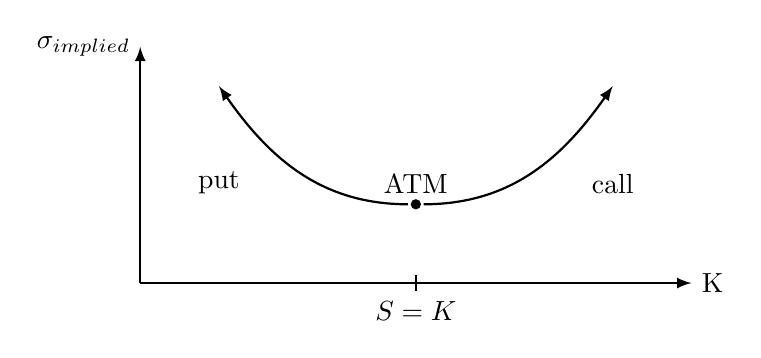
\begin{tikzpicture}[thick]
    \draw [-latex] (0,0) to (7,0) node [right] {K};
    \draw [-latex] (0,0) to (0,3) node [left] {$\sigma_\text{implied}$};
    \draw [-latex] (3.6,1) to [out=0,in=-125] (6,2.5);
    \node [above] at (6,1) {call};
    \draw [-latex] (3.4,1) to [out=180,in=-55] (1,2.5);
    \node [above] at (1,1) {put};
    \draw [fill] (3.5,1) circle [radius=0.05] node [above] {ATM};
    \draw (3.5,0.1) to (3.5,-0.1) node [below] {$S=K$};
\end{tikzpicture} \\

This shape became known as a {\em smile}. There was no theoretical basis for this change, only empirical observation, and practitioners looked for an interpretation. The market realised that the seller of the option charged a higher volatility because big moves were more likely to occur than in the Black-Scholes representation. \\

By 1984, it was widely recognized that the divergence of the model with emprical observation needed to be addressed. In 1987, several papers (Wiggins, Johnson and Shanno, Hull and White) introduced stochastic volatility into option pricing. The Hull and White model was formulated as follows:
\begin{align*}
\text{under}& \Pmeas & \frac{\dif S(t)}{S(t)} &= \mu \dif t + \sigma(t) \dif W^1(t) \\
 \text{and}& & \frac{\dif \sigma(t)}{\sigma(t)} &= a \dif t + \xi \dif W^2(t)
\end{align*}
Where $\dif W^1, \dif W^2$ are correlated: $\dif W^1(t) \dif W^2(t) = \rho \dif t$. \\

If $S$ is a stock, then $\rho$ should be negative; as the stock goes down, the volatility rises, because the equity of a firm decreases, while the debt remains the same. This is known as the {\em leverage effect}.
















\end{document}
